\label{sec:pathselection}

In this chapter, we will describe what Path Selection (PS) is, how it works and which strategies we use to take advantage of multiple computed paths per agent. Figure~\ref{fig:overview_merging} shows the different steps for Path Selection used in this work.

\begin{figure}[H]
    \centering
    \caption{Overview of Path Selection}\label{fig:overview_merging}
    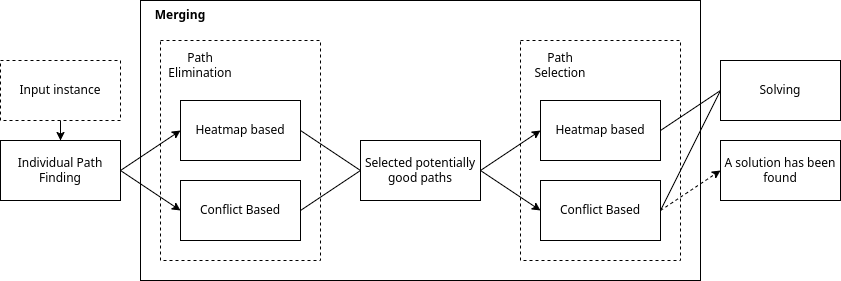
\includegraphics[width=\widthimg]{img/overview_merging.drawio.png}
\end{figure}


Path Selection takes a \(\tau\) as its input and produces a subcomponent \(\tau'\) when \(\forall a \in A \text{ } | \text{ } \gamma'_a \in \tau' \subseteq \gamma_a \in \tau\). Furthermore \(\tau'\)  denotes a plan, where \(\forall \gamma'_{a \in A' \subseteq A}\in \tau',| \gamma'_a|=1 \). 


\section{Heatmap}

Heatmap is about projecting likelihood of presence of an agents on vertices at each step. Inspired from papers~\cite{atstfestko20a, banatu02a}. Likelihood refers to, in a scope of an agent, the probability of be being at a specific vertex for each time step according to a set of path \(\gamma\). This heatmap interpretation stands for the scope of one agent. We will refer to single agent heatmap as \textbf{Individual Heatmap} (IH). We formalize, in equation~\ref{math:individual_heatmap} an Individual Heatmap function:

\begin{equ}[H]
    \begin{equation}\label{math:individual_heatmap}
        \phi(\gamma,v,t) = \frac{| \{\pi|\pi \in \gamma,\pi(t) = v\}|}{|\gamma|}
    \end{equation}
    \caption{Individual Heatmap}
\end{equ}


\(\phi\) is calculated --  given a \(\gamma\) of an agent, a vertex and a timepoint. For example, we can compute the Individual Heatmap of a given \(|\gamma|=3\) illustrated in figure~\ref{fig:individual_heatmap}.

\begin{figure}[H]
    \centering
    \caption{Example of Individual Heatmap computed from a \(|\gamma|=3\)}\label{fig:individual_heatmap}
    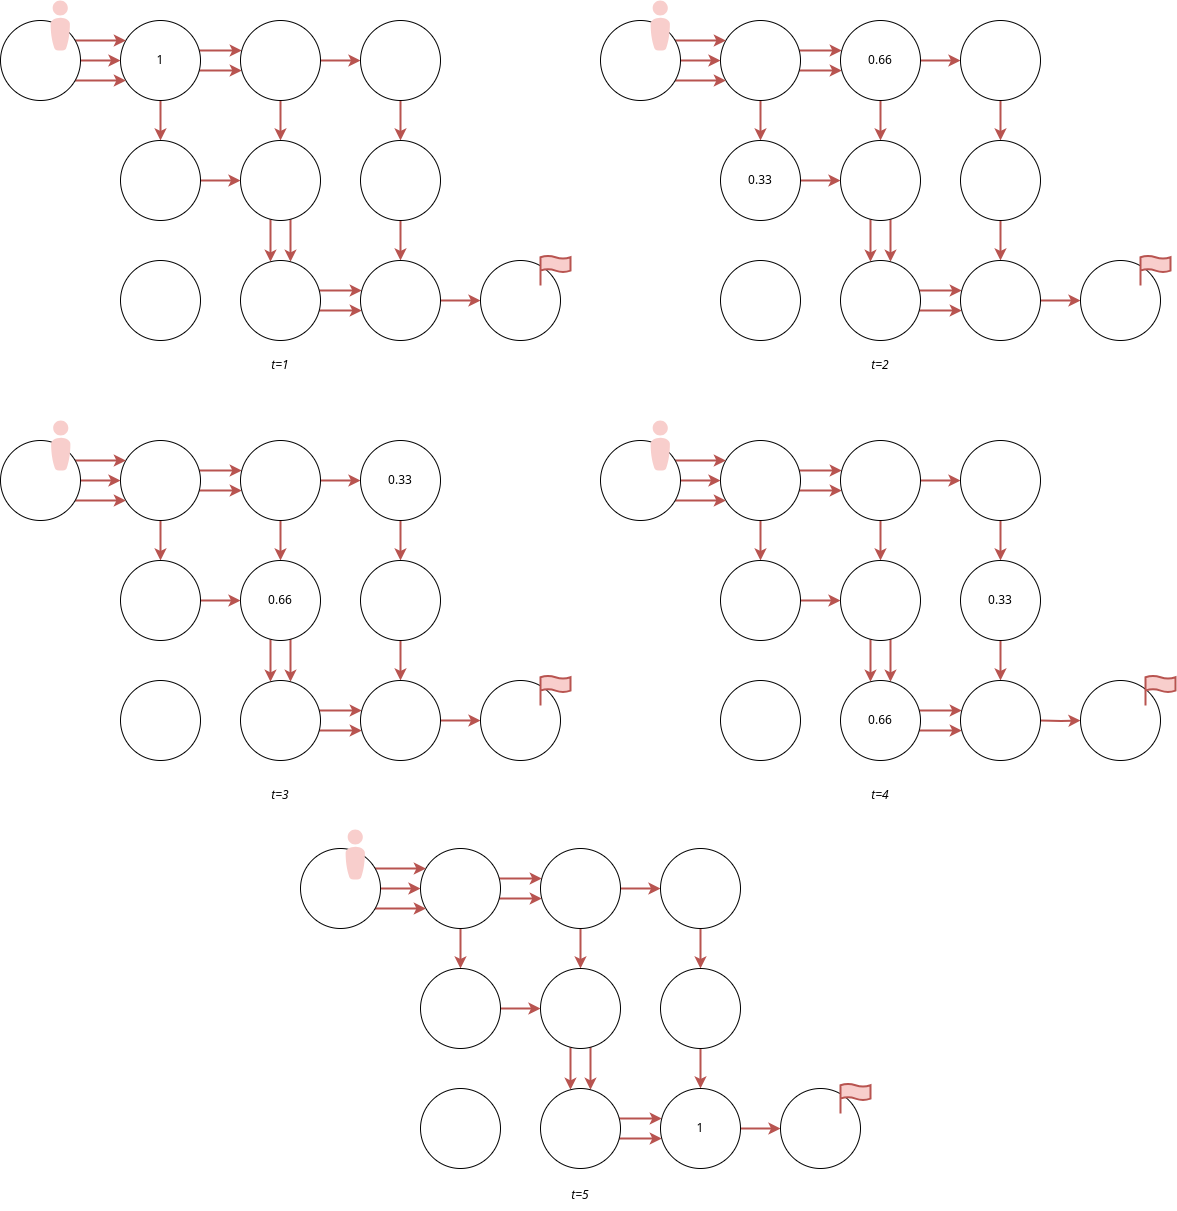
\includegraphics[width=\widthimg]{img/individual_heatmap.drawio.png}
\end{figure}

This representation produces critical vertices for an agent, where higher values correspond to a greater likelihood of vertex utilization. On the other hand, the mean heatmap value associated with \(\gamma\) serves as an indicator of path diversity, with elevated values signifying a low level of path diversity.

we derive a \textbf{Global Heatmap} (GH) through the aggregation of all Individual Heatmaps. It is important to note that Global Heatmaps, in this context, no longer serve as a direct indicator of the likelihood of presence but instead an indicator of ``usage of vertices'' .

A Global Heatmap \(\Phi\) of \(\tau\) is formalized in the following equation~\ref{math:global_heatmap}. As for Individual Heatmaps, a Global Heatmap value of \(\Phi\) is computed given a vertex \(v\) and a time step \(t\).  

\begin{equ}[H]
    \begin{equation}\label{math:global_heatmap}
        \Phi(\tau,v,t) = \frac{ \sum_{\gamma \in \tau}\phi(\gamma,v,t)}{|\tau|}
    \end{equation}
    \caption{Global Heatmap}
\end{equ}


To perform the computation of Individual Heatmaps and Global Heatmaps using Clingo, it is important to consider that Clingo inherently rounds down floating-point numbers. To obtain accurate heatmaps values in our context, we require an external program capable of performing divisions without rounding down the result.
We introduce the encoding of the Individual Heatmap in listing\ref{lst:individual_heatmap_encoding}.

\begin{minipage}[H]{\linewidth}
\begin{lstlisting}[style=mystyle, caption={Individual Heatmap encoding}, label={lst:individual_heatmap_encoding}]
    individual_heatmap(R,V,T,(K,N)) :- 
        K = #count{1,I : at(R,I,V,T)}, |\label{line:ihm_counting_paths}|
        N = #count{1,I : at(R,I,_,_)}, |\label{line:ihm_counting_all_paths}|
        at(R,_,V,T).  
\end{lstlisting}
\end{minipage}


This short encoding introduces  \(heatmap/4\) predicates, with \(R\), \(V\) and \(T\) being respectively the agent ID, a vertex and a time point. The last argument of the predicate is a tuple \((K,N)\) where \(K\), computed on line~\ref{line:ihm_counting_all_paths}, is the number of paths of \(R\) that go through \(V\) at time step \(T\). And \(N\), computed on line~\ref{line:ihm_counting_all_paths}, denotes the number of paths that belong to the agent \(K\).

The calculation of the Global Heatmap is performed using \textbf{Python}\footnote{It is possible to provide the nominator and the denominator for the Global Heatmap at each vertex and each time step, however, compared to using a third-party programming language, it is very slow or not computationally feasible in practice.}.


\section{Path Elimination}

Path Elimination (PE) is the process of the removing paths that exhibit potential issues. It serves to chunk through the multitude of possible paths and eliminate those that are deemed ``potentially problematic''. This step serves as a preprocessing stage for Path Selection (PS). 

Figure~\ref{fig:overview_merging_path_elemination} sums up the different processes in order to eliminate potentially-conflicting-paths.

\begin{figure}[H]
    \centering
    \caption{Overview of Merging: Path Elimination}\label{fig:overview_merging_path_elemination}
    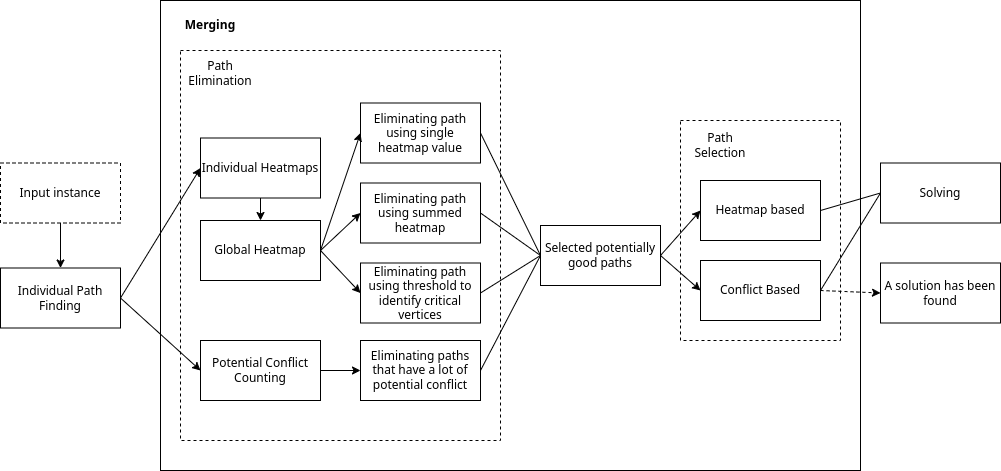
\includegraphics[width=\widthimg]{img/overview_merging_path_elimination.drawio.png}
\end{figure}

We first introduce some definition.

\begin{definition}
    A path is classified as \textbf{killed} when it has been explicitly removed of the output of Path Elimination.
\end{definition}

\begin{definition}
    A path is classified as \textbf{selected} when it has been explicitly selected for the output of Path Elimination.
\end{definition}

\begin{definition}
    An agent is classified as \textbf{killed} when all of its paths have been explicitly killed during the Path Elimination process.
\end{definition}

\begin{definition}
    A vertex can be classified as \textbf{critical} at a certain time step by a Path Elimination process. It assume that there is high chance of collision.
\end{definition}

\begin{definition}
    An agent is classified as \textbf{critical} when at least one of the vertices composing its plan is considered as \textbf{critical} in each of its paths.
\end{definition}

\begin{definition}
    A \textbf{potential conflict} denotes conflict among paths of different \(\gamma\). It do not represent an actual conflict.
\end{definition}



\subsection{Using Global Heatmap}

Global Heatmap values often provide insights into vertices that are prone to conflicts. This information can be leveraged for path elimination. 

A simplistic approach involves minimizing the cumulative Global Heatmap value by allowing the encoding select or not paths for the computation of GH. Unfortunately, due to the interconnections among heatmaps, practical grounding of this approach becomes feasible only on small instances.

We then present three approaches for identifying potentially conflicting paths in a reasonable computation time.

\subsubsection{Eliminating paths using unique heatmap value}

One straightforward approach involves ordering all possible assignments of \((v, t)\) within a given \(\tau\) based on their global heatmap values. We classify the top \(k\) vertices as ``critical''.Which can then be used as reference points for path elimination based on various criteria. We can identify which paths pass through critical vertices using the following rule:

\begin{minipage}[H]{\linewidth}
\begin{lstlisting}[style=mystyle]
    critical_path(R,I,V,T) :- 
        critical_vertex(V,T), 
        at(R,I,V,T), 
        not path_killed(R,I).
\end{lstlisting}
\end{minipage}


We then determine \(n\) critical paths that should be eliminated. For instance, we may opt to eliminate half of them as follows:

\begin{minipage}[H]{\linewidth}
\begin{lstlisting}[style=mystyle]
    {to_kill(R,I): critical_path(R,I,V,T) } = K/2 :-
        K = #count{1,R',I' critical_path(R',I',V,T)},
        critical_vertex(V,T).
\end{lstlisting}
\end{minipage}

Note that we use predicate\(to\_kill/2\) and \(path\_killed/2\) that refer to the same concept. We do differentiate them so the paths that are yet to be eliminated (\(to\_kill/2\)) do not interfere with already killed paths (\(path\_killed/2\)).  

There are various parameters and variations to consider in determining the value that \(n\) can take. These may include individual heatmap values, whether an agent has already had some of its paths eliminated

The approach we settle on is the following;

\begin{figure}[H]
    \centering
    \caption{Eliminating paths using unique heatmap value}\label{fig:simple_heatmap_value_elimination}
    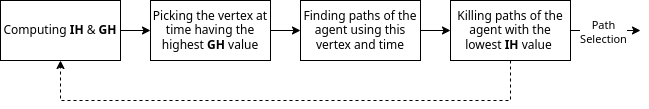
\includegraphics[width=\widthimg]{img/simple_heatmap_value.drawio.png}
\end{figure}

As illustrated in figure~\ref{fig:simple_heatmap_value_elimination}, it is possible to loop the process to eliminate more paths. 

As mentioned earlier, the lack of floating-point number handling of Clingo forces us to use a Python wrapper to sort Global and Individual Heatmap values.

The decision to eliminate paths of agents with the lowest Individual Heatmap values can be justified on two grounds:
\begin{enumerate}
    \item \textbf{Node Importance}: Higher Individual Heatmap values signify that a particular vertex holds more significance at this time step for the respective agent. Consequently, it is more suitable to eliminate paths of agents with lower interest in this vertex, as they are less likely to utilize it.
    \item \textbf{Balanced Elimination}: Opting to eliminate paths of agents with low Individual Heatmap values helps maintain a balanced elimination process; selecting agent with the lowest heatmap means killing the least possible paths involved in the \textbf{critical vertex}. It allows us to not kill agents too swiftly. 
\end{enumerate}

If we apply the previous approach explained above, on the example illustrated on figure ~\ref{fig:ipf_example}. We highlighted global heatmap in red at the critical moment (time step \(t=3\)), see figure~\ref{fig:simple_heatmap_value_elimination_example}. 

\begin{figure}[H]
    \centering
    \caption{Eliminating paths using unique Global Heatmap value process example}\label{fig:simple_heatmap_value_elimination_example}
    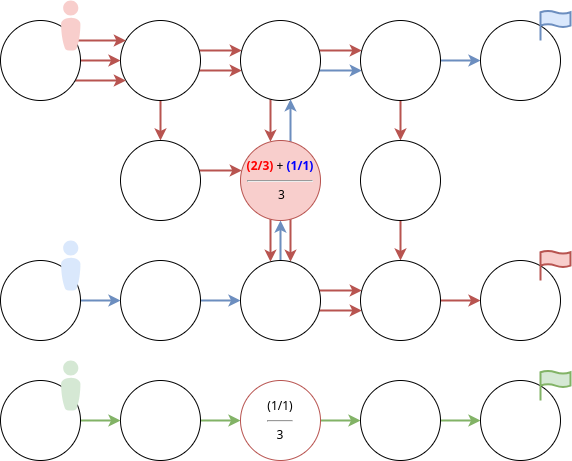
\includegraphics[width=\widthimg]{img/pe_one_heatmap_value_example.drawio.png}
\end{figure}

Between the two highlighted vertices, according to the elimination process~\ref{fig:simple_heatmap_value_elimination}, the vertex with the highest Global Heatmap value is the one colored in red. From this vertex, we can denote three paths going through it at time step \(t=3\). We then order the Individual Heatmap values of the two concerned agents, blue and red. from these values we can deduce that the two paths of red agents have to be killed. We obtain figure~\ref{fig:simple_heatmap_value_elimination_example} which is in this case a valid plan:

\begin{figure}[H]
    \centering
    \caption{Result of eliminating paths using unique heatmap value process}\label{fig:simple_heatmap_value_elimination_example_result}
    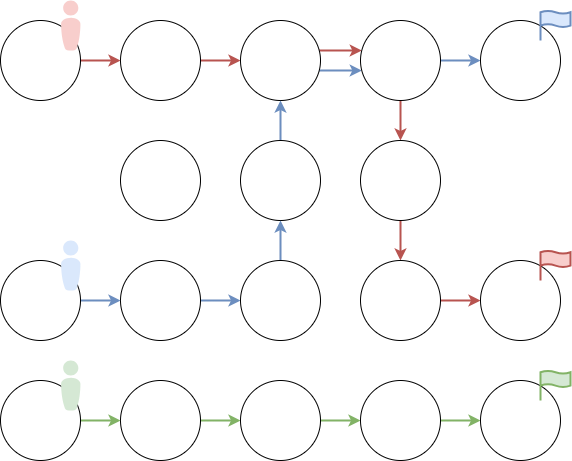
\includegraphics[width=\widthimg]{img/pe_one_heatmap_value_example_result.drawio.png}
\end{figure}

Nevertheless, despite our efforts to implement strategies aimed at balancing the elimination process among agents, adopting a vertex-oriented approach tends to kill agents swiftly.

\subsubsection{Eliminating paths using GH threshold}

One flaw that comes with the previous approach is that the process is doing one vertex after an other. It is difficult to define a value that eliminate the right amount of paths to be relevant. We propose a way to identify multiple critical vertices in one call.

The principle is simple, if the Global Heatmap value of a vertex at a specific time point is higher than a defined value \(\mathcal{H}\), the vertex is denoted as critical. We call this defined value a \textbf{threshold}. Formally, we have;

\begin{equ}[H]
    \begin{equation}\label{math:critical_vertex_threshold}
        critical\_vertices(\tau) = \{(v,t) | \Phi(\tau,v,t) > \mathcal{H}, (v,t) \in \mathcal{F}(\tau) \} 
    \end{equation}
    \caption{Identifying critical vertices using threshold}
\end{equ}

Where \(\mathcal{F}\) is a function enumerating all possible tuple \(v,t\) in \(\tau\):

\[
    \mathcal{F}(\tau) = \mathlarger{\mathlarger{\bigcup_{\gamma\in\tau}}}\bigcup_{\pi\in\gamma}\cup_{t=0}^{t \rightarrow |\pi|}{(\pi[t],t)}
\]


Threshold values can be defined through different equations, considering different properties. Equation~\ref{math:simple_biased_threshold}, denoted as \(\mathcal{H}_{sbt}(A,\Delta)\), defines a simple biased threshold. In essence, without considering the bias, this equation implies that a vertex is labeled critical if, for all \(n\) agents with \(k\) paths each, \(\frac{1}{n}\) of their paths utilize this vertex at a specific time plus one additional path. The bias adjustment allows for the flexible inclusion of more or less critical vertices.

\begin{equ}[H]
    \begin{equation}\label{math:simple_biased_threshold}
        \mathcal{H}_{sbt}(A,\Delta) =  \frac{1*\Delta}{|A|}
    \end{equation}
    \caption{Simple (biased) threshold}
\end{equ}



The simplicity of the basic threshold equation makes it a general tool, but it lacks vertex-specific context. To address this limitation, we introduce a more sophisticated approach with a context-dependent threshold in equation~\ref{math:contextdependant}. This threshold calculation takes into account the number of paths using a particular vertex at a specific time step (\(T\)) and the number of agents involved, providing a more precise evaluation of critical vertices. The equation incorporates a bias factor \(\Delta\) that is used for finetuning.

\begin{equ}[H]
    \begin{equation}\label{math:contextdependant}
        \mathcal{H}_{bcdt}(V,T,A,\Delta) = \frac{npath\_on(V,T)*\Delta}{nagent\_on(V,T) * |A|}
    \end{equation}
    \caption{(Biased) Context dependent threshold}
\end{equ}


\subsubsection{Eliminating paths using sums of heatmap values}

In contrast to a vertex-oriented approach, which may label a path as "critical" even if it possesses critical attributes only on a single occurrence. An alternative strategy involves considering the scope of entire paths that may highlight conflict. The approach entails assigning a value to an entire path by summing the Global Heatmap values associated with its vertices. The approach is outlined in figure~\ref{fig:summed_heatmap_value_elimination}. 

\begin{figure}[H]
    \centering
    \caption{Eliminating paths using summed Global Heatmap values process overview}\label{fig:summed_heatmap_value_elimination}
    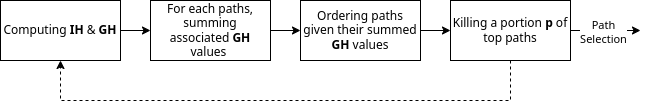
\includegraphics[width=\widthimg]{img/summed_heatmap_value.drawio.png}
\end{figure}

This approach tends to kill agents quite quickly when only a few paths are involved. However, it tends to be more efficient the more diverse \(\gamma\in\tau\) are. Futhermore, with one call, this approach can chunk a significant portion of the paths. 


\subsection{Using conflicts}

We introduce a fourth approach that centers around \textbf{potential conflicts} to guide Path Elimination. In this method, for each agent and at every vertex along their path, we calculate the count of \textbf{potential conflicts}. This approach stands apart from the heatmap-based methods in a significant way: when an agent possesses a substantial number of paths, their individual paths do not significantly influence the Global Heatmap values, even if they have the potential to cause conflicts. However, in the Potential Conflict-based approach, every path is treated with equal weight.

The encoding for the described approach is defined in Listing~\ref{lst:conflict_based_path_elimination}.


\begin{minipage}[H]{\linewidth}
\begin{lstlisting}[style=mystyle, caption={Conflict-based Path Elimination}, label={lst:conflict_based_path_elimination}]
    #const n = 5.

    to_determine(R,I) :- at(R,I,_,_), not path_killed(R,I). |\label{line:to_determine}|

    potential_conflict(R,I,V,T) :- |\label{line:potential_conflict}|
        to_determine(R,I), at(R,I,V,T), 
        to_determine(R',I'), at(R',I',V,T), 
        R'!=R.

    path_composition(R,I,C) :- |\label{line:path_composition}|
        C = #count{1,V,T : potential_conflict(R,I,V,T)}, 
        to_determine(R,I).

    {to_kill(R,I,C): path_composition(R,I,C)} = n. |\label{line:to_kill_set}|

    #maximize {C:to_kill(_,_,C)}. |\label{line:maximize_to_kill}|
\end{lstlisting}
\end{minipage}

In order to decide which paths have to be killed, we first need to identify which paths can be killed. Line~\ref{line:to_determine} labels paths with the predicate \(to\_determine/2\). \textbf{Potential conflicts} are determined through the rule at line~\ref{line:potential_conflict}. This rule identifies situations where two or more agents could potentially conflict at a given vertex and time. Rule at line~\ref{line:path_composition} calculates the number of \textbf{potential conflicts} composing it. Finally, lines~\ref{line:to_kill_set} and~\ref{line:maximize_to_kill} state that exactly \(n\) paths should be marked for elimination and aims to select the set of paths to eliminate that results in the highest \textbf{potential conflicts} sums. Note that \(n\) has been set arbitrarily to 5, but it can take any value.  

\section{Path Selection}\label{sec:ps}

As mentioned above, Path Selection tends to build a \(\tau' \leq \tau\). We can describe two objectives for \(\tau'\).  

1). Building \(\tau'\) in order to create a plan. We can identify two kinds of plans; a valid plan \(\Pi\) as defined earlier in the background section~\ref{sec:background}, and a partial plan \(\hat{\Pi}\). A partial plan possesses the same attributes as a valid plan, but only for a subset of the agents. This means that  for each \(\gamma' \in \tau', |\gamma'| \leq 1\). 

2). Building \(\tau'\) in order to create a subgraph. We create a subgraph \(V',E'\) build out of the paths in \(\tau'\). We have 
\(V' = \{v \text{ }|\text{ } v \in vertices(\tau')\} \)  and \(E' = \{e \text{ }|\text{ } e \in edges(\tau')  \} \) where \(vertices(\tau)\) and \(vertices(\tau)\) respectively enumerate the vertices and edges of a given set of set of path \(\tau\). This means that  each \(\gamma' \in \tau', |\gamma'|  \geq 1 \). 


\begin{figure}[H]
    \centering
    \caption{Overview of Merging: Path Selection}\label{fig:overview_merging_path_selection}
    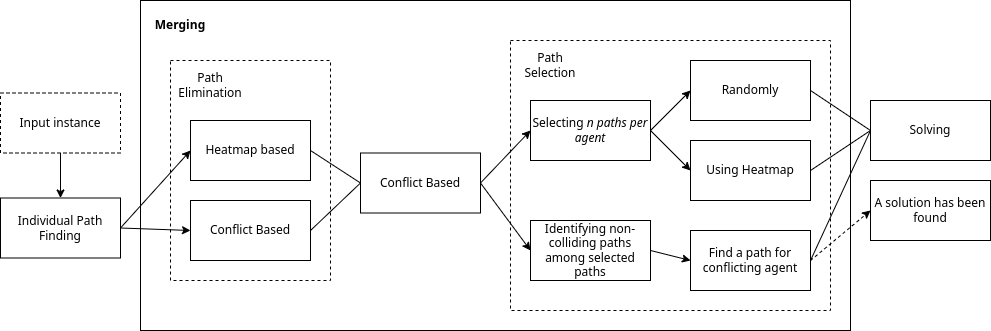
\includegraphics[width=\widthimg]{img/overview_merging_path_selection.drawio.png}
\end{figure}



\subsection{Towards a (partial) plan}

In this section, we explain the method for achieving the first objective outlined above. To summarize, the aim is to identify a partial plan \(\hat{\Pi}\) with the maximum amount of agents.  The corresponding encoding for this approach is provided in Listing~\ref{lst:ps_encoding}.

\begin{minipage}[H]{\linewidth}
\begin{lstlisting}[style=mystyle, caption={Building a conflict free \(\tau'\)}, label={lst:ps_encoding}]
    % Defining collision & possible_path
    possible_path(R,I):- at(R,I,_,_), not path_killed(R,I). |\label{line:possible_path}|
    
    % Constructing a (partial) plan
    {selected_path(R,I) : possible_path(R,I) }1 :-  agent(R). |\label{line:selecting_candidate}|

    collision((R1,P1),(R2,P2),T) :- |\label{line:vertex_collision}|
        R1 != R2, at(R1,P1,V,T), at(R2,P2,V,T),
        selected_path(R1,P1), selected_path(R2,P2).

    collision((R1,P1),(R2,P2),T) :- |\label{line:edge_collision}|
        R1 != R2, at(R1,P1,V1,T), at(R1,P1,V2,T+1), at(R2,P2,V2,T), 
        at(R2,P2,V1,T+1), selected_path(R1,P1), selected_path(R2,P2).
    
    :- collision((R1,P1),(R2,P2),_), |\label{line:no_collision}|
        selected_path(R1,P1), 
        selected_path(R2,P2).

    selected_agent(R) :- selected_path(R,_).  |\label{line:select_agent}|    

    #maximize {1@1,R : selected_path(R,_)}. |\label{line:more_agent}|
\end{lstlisting}
\end{minipage}

Up to this step of Path Selection, paths could have been labeled as either \textbf{selected} or \textbf{killed}. For the remaining paths, line~\ref{line:possible_path} labels them as \(possible\_path/2\). Then, line~\ref{line:selecting_candidate} selects paths from the candidates, ensuring that at most one path per agent is chosen for the output. Following this, lines~\ref{line:vertex_collision} and~\ref{line:edge_collision} define vertex and edge collisions, respectively, among the selected paths. The associated constraint specified in line~\ref{line:no_collision} ensures that the set of \textbf{selected paths} does not contain any collisions. Lastly, the optimization statement in line~\ref{line:more_agent} aims to maximize the number of \textbf{selected paths}, ensuring the selection of as many paths as possible.


\subsection{Towards a subgraph}

The second objective discussed in~\ref{sec:ps} can defined as a pre-processing for a MAPF algorithm. Contrary to the first objective, we require at least one path for each agent. To do so, multiple approaches can be used. By definition, the output of IPF can be used directly. We will, however, describe different approaches to select some paths per agent. 

The approaches that we describe are based on the output of the encoding described in Listing~\ref{lst:ps_encoding}.
The objective is to populate the set of conflict-free paths with paths of agents involved in conflicts. We define two primary approaches:

\noindent\textbf{Utilizing Global Heatmaps:} The first approach involves using GH and similar approaches used in Path Elimination process. This can be done either by employing the Heatmaps computed during the Path Elimination process or by recalculating them using the possible paths issued from~\ref{lst:ps_encoding}  (or from IPF, if all paths have been eliminated)..

\noindent\textbf{Path Conflict Composition:} The second approach relies on path conflict composition, as outlined in Listing~\ref{lst:conflict_based_path_elimination}. Similarly to the heatmap approach, the path conflict composition can be derived either from the Path Elimination process or can be recomputed based on the possible paths obtained through path selection.


We then convert the different paths into the new vertices and edges using the following encoding~\ref{lst:converting_paths_to_subgraph}.

\begin{minipage}[H]{\linewidth}
\begin{lstlisting}[style=mystyle, caption={Converting path to subgraph}, label={lst:converting_paths_to_subgraph}]
    nvertex(V) :- selected_path(R,I), at(R,I,V,_).
    nedge(U,V) :- 
        edge(U,V), 
        nvertex(U), 
        nvertex(V).
\end{lstlisting}
\end{minipage}


\subsection{Evaluating approaches}

We introduced different Path Elimination approaches coupled with Path  Selection, in order to evaluate them, we introduce four metrics. These metrics require a reference to compare Path Selection efficiency. We then introduce a ``brute-force'' Path Selection approach that computes what could be defined as the best output possible for Path Selection\footnote{In our case, the best output possible is a partial plan \(\hat{\Pi}\) as close as possible to a complete valid plan \(\Pi\)}.  This approach is not used in practice because of its huge computation time.


\begin{minipage}[H]{\linewidth}
\begin{lstlisting}[style=mystyle, caption={``Brute-force'' PS approach}, label={lst:brut_force_ps_encoding}]
    % Defining collision & possible_path
    collision((R1,P1),(R2,P2),T) :- 
        R1 != R2, 
        at(R1,P1,V,T), 
        at(R2,P2,V,T).

    collision((R1,P1),(R2,P2),T) :- 
        R1 != R2, 
        at(R1,P1,V1,T), 
        at(R1,P1,V2,T+1), 
        at(R2,P2,V2,T), 
        at(R2,P2,V1,T+1).

    possible_path(R,I):- at(R,I,_,_).

    % Constructing set of non conflicting paths
    {usable_path(R,I) : possible_path(R,I) } :- agent(R).

    :- collision((R1,P1),(R2,P2),_), 
        usable_path(R1,P1), 
        usable_path(R2,P2).

    :- selected_path(R,I), not usable_path(R,I).

    % Constructing a partial plan
    {selected_path(R,I) : possible_path(R,I) }1 :- agent(R).

    :- collision((R1,P1),(R2,P2),_), 
        selected_path(R1,P1), 
        selected_path(R2,P2).

    #maximize {1@1,R : selected_path(R,I)}.
    #maximize {1@2,R,I : usable_path(R,I)}.

\end{lstlisting}
\end{minipage}

The major reason for the long computation time required by the ``brute-force'' PS approach is the identification of vertex and edge conflicts.

We introduce metrics to assess and compare the outcomes of various Path Selection approaches. We will compare the results of approaches to the brut-force output. To do so, we introduce two functions \(brutforce\) and \(approach\) which both take as argument a predicate name and return the associated set of facts. For instance, \(approach(selected\_path/2)\) returns all the selected paths of the approach in a tuple form.

\begin{equ}[H]
    \begin{equation}\label{math:relevance}
        relevance = \frac{|approach(selected\_agent/1) \cap brutforce(selected\_agent/1)|}{|approach(selected\_agent/1) \cup brutforce(selected\_agent/1)|}
    \end{equation}
\caption{Relevance}
\end{equ}

\textbf{Relevance} computes the proportion of common selected agent designated by the approach with brutforce output.

\begin{equ}[H]
    \begin{equation}\label{math:absolute_relevance}
        absolute\_relevance = \frac{|approach(selected\_agent/1)|}{|approach(agent/1)|}
    \end{equation}
\caption{Absolute Relevance}
\end{equ}

\textbf{Absolute Relevance} evaluates the proportion of conflict-free agents found by the approach.


\begin{equ}[H]
    \begin{equation}\label{math:precision}
        precision = \frac{|approach(selected\_path/2) \cap brutforce(usable\_path/2)|}{|approach(selected\_path/2) \cup brutforce(usable\_path/2)|}
    \end{equation}
\caption{Precision}
\end{equ}

\textbf{Precision} evaluate capacity of the approach to select path that are present in the biggest set of conflict-free paths possible. 

\begin{equ}[H]
    \begin{equation}\label{math:chunk_proportion}
        chunk_proportion = \frac{|approach(path\_killed/2)|}{|brutforce(possible\_path/2)|}
    \end{equation}
\caption{Chunk Proportion}
\end{equ}

\textbf{Chunk Proportion} evaluate the proportion of path killed compared to the number of paths. 

